This Appendix is to describe the raster calibration that I performed for the tritium family of experiments. When performing the calibration, the traditional method did not work due to some unforeseen problems with the Beam Position Monitors inaccurately reporting the full beam spread. This issue led me to develop a new way to calibrate the raster should this issue arise for a future experiment. I have written a technical note for Hall A documenting this procedure \cite{MyRaster}. The rest of this Appendix is a subset of the technical note that focuses on the important details for performing the calibration.

\label{app:raster_cal}
\section{What is a Raster Calibration} \label{what}

A well calibrated raster will map a raster current to the instantaneous beam position at both Beam Position Monitors (BPMs) and the target. Accurate beam position data is critical for proper reconstruction of the reaction vertex of physics events. A poorly calibrated horizontal raster will cause poor z-vertex resolution, making it more difficult to subtract the background from target endcaps. A poorly calibrated vertical raster will incorrectly reconstruct event momentum, causing errors in physics analysis.

%The raster calibration can be thought of as defining a line that maps the raster current (measured in ADC bins) to a position.

The raster calibration is completed by defining a function to map the raster current (measured in ADC bins) to a position. The default raster class in the Hall A analyzer uses a linear function for the calibration. Each coil will have two calibration values per position: the slope and intercept of this line. When running in single-arm mode, each raster needs to be calibrated for each arm independently. This is because of differences in performance of the ADCs on each arm. This give a total of twenty-four calibration values as there are three positions (two BPMs and the target) and four coils (two per dimension) calibrated for two arms. When running in coincidence mode, the calibration only needs to be done once since only one arm records the beam data that is used. In this case, there are twelve calibration values. The slope of the line determines the size calibration of the raster coil, the value converts the raster current (in ADC units) to a beam position displaced about the mean beam position. The intercept of the line, in conjunction with the slope, sets this mean beam position. The slope should have units of $meters(m)/$\textit{ADC bin} and the intercept should have units of $meters$.

The Hall A Analyzer software has the capability to include correlation between the x (y) position and the y (x) raster. Historically, this has not been used. There is no evidence that such a correlation exists. This would only come into play if the raster magnets were to shift off-axis (i.e. they rotate so that an electron moving in the z-direction is deflected in a direction that is not purely horizontal or vertical).

The calibration is applied through matrix arithmetic. The raster currents (measured in \textit{ADC Bins}) are represented as a $1\times2$ row matrix. This is then multiplied by the \textit{ADC Bin} to $m$ conversion factor matrix (the slopes of the calibration). This is a $2\times2$ matrix that would only have non-zero off-diagonal elements in the case of an off-axis raster correlation. Finally, the $1\times2$ offset matrix is added to get the final $1\times2$ position matrix.

Equation \ref{cal_apply} shows how the Hall A Analyzer software applies the calibrations. In this equation $R$ represents the raster current, $S$ represents the conversion factor, and $O$ represents the offset. The $l$ indices represent the location of the calibration (i.e. ``A'' for BPMA, ``B'' for BPMB, and ``T'' for target).

\begin{equation}
	\begin{bmatrix}
		^lx & ^ly
	\end{bmatrix}
	=
	\begin{bmatrix}
		^lR_x & ^lR_y
	\end{bmatrix}
	\times
	\begin{bmatrix}
		^lS_{xx} & ^lS_{xy} \\
		^lS_{yx} & ^lS_{yy}
	\end{bmatrix}
	+
	\begin{bmatrix}
		^lO_x & ^lO_y
	\end{bmatrix}
	\label{cal_apply}
\end{equation}

The position at the target is used to determine where the beam is at when intersecting the $z=0$ plane (target center). The positions at the BPMs are used to determine the trajectory of the beam (i.e. at what angle is the beam intersecting the $z=0$ plane). When combined with the interaction plane defined by HRS tracking, the true reaction point can be found. This increases the accuracy of physics reconstruction.

Since only one set of coils is used for physics analysis, that is the only set that is \textit{required} to be calibrated. The method for calibrating the beam position at the target described in this document can only be applied to that particular set of coils. For the Tritium experiments, we used the ``traditional'' method to calibrate the unused set of coils. This was an unnecessary step, as they were never used in analysis; this was done to give us a good starting point in case some unforeseen error required their use.

The second set of coils could be calibrated in this same way by modifying the Rastered Beam class (\textit{THaRasteredBeam}). The data used for physics reconstruction is defined by the THaDetector type class that is added first. By recompiling the analyzer after changing the first raster added, the following calibration methods can be employed for the second set of coils.\cite{Gen}

\section{Determining the Sign of the Calibration}

When determining the beam position, it is obvious to look at the BPM. These are sets of sensing wires in the beamline that can measure the beam position. While the position of the beam reported by the BPMs is highly accurate when averaged over time, the measurement is a slow process and cannot be used on an event-by-event basis. This slowness can cause misleading interpretations of beam movement if we are not careful.

The raster current measures displacement about the central beam position. This measurement says nothing about the \textit{direction} of the displacement. To determine this relation, which is critical to calibrating the rasters, we must use the BPMs and a fixed position feature that we can see in both the BPM and raster spectra: The Carbon Hole target.

To begin, the Carbon Hole must be visible to the beam. Machine Control Center (MCC) is then asked to steer the beam to another BPM position, changing only one dimension. Once there, a short run is taken using the clock trigger. By observing how the carbon hole has moved in the BPM spectrum, the direction that the beam moved can be determined. Note that the MCC BPM coordinate system is not always the same as the hall coordinate system; the BPM data recorded by the Data Acquisition System (DAQ) is in the hall coordinate system. By then observing how the carbon hole moves in the raster spectrum, it can be determined if the coordinate system of the raster in that dimension is the same as that of the BPMs. If the direction of the movement is the same, the sign of the calibration in that dimension is $1$; if the movement is opposite, the sign is $-1$.

This procedure must be completed for both the horizontal and vertical dimensions. The results of this procedure should not change unless the raster power supplies are worked on and wired differently. Under typical circumstances, an experiment only needs to do this procedure once. For the Tritium experiments, we found the sign of the horizontal calibration to be $1$ and the sign of the vertical calibration to be $-1$.\cite{Dien}

\section{Calibrating the Beam Position on Target}

In the past, the calibration values have been found by assuming that the BPMs accurately reflect the mean position and overall magnitude of the rastered beam. By mapping the mean and RMS of raster current to the mean and RMS of BPM positions, a 1:1 mapping could be quickly achieved. Unfortunately, a bandpass filter on the BPM signal prevents the BPMs from accurately reproducing the full size of the rastered beam. We aim to improve on this method to provide the most accurate picture of the beam spread that we can.\cite{bpm_slow}

%Unfortunately, in the Tritium era of Hall A, we have seen that the BPMs no longer accurately reflect the magnitude of the rastered beam. An explanation of this behavior has not been found. Nevertheless, we must find a new calibration method.

While the BPMs can (and still are) used to determine the mean beam position, we must look for other quantities to calibrate the raster size. The obvious choice is the carbon hole target. The carbon hole is used to set the size during data taking because it is known to have a diameter of 2mm. The hole is visible in the raster spectrum, so we can fit it to determine a size calibration for the raster.

The resolution of reconstructed events does not allow for a hard line between the events originating from the foil and the absence of events in the ``hole'' region. Events smear across this border suggesting that we ought to use a smooth function to define the edge. We decided to use a radial sigmoid function with a floating ``hardness'' constant. A sigmoid, shown in equation \ref{eqn:base_sig}, is a smoothed step function with a constant that determines how hard of a step it is. In this general form of the equation, $a$ is the vertical axis and $b$ is the horizontal axis. As shown in Figure \ref{fig:sighard}, a sigmoid approaches a step function as the ``hardness'' constant approaches infinity. This was found to converge\footnote{When doing these fits, be sure to the Log Likelihood method} and visually appears to fit the hole well. This fitting procedure determines the edge of the hole to be at the position where the value is halfway between the minimum and maximum value of function.\cite{Evan}

\begin{figure}
	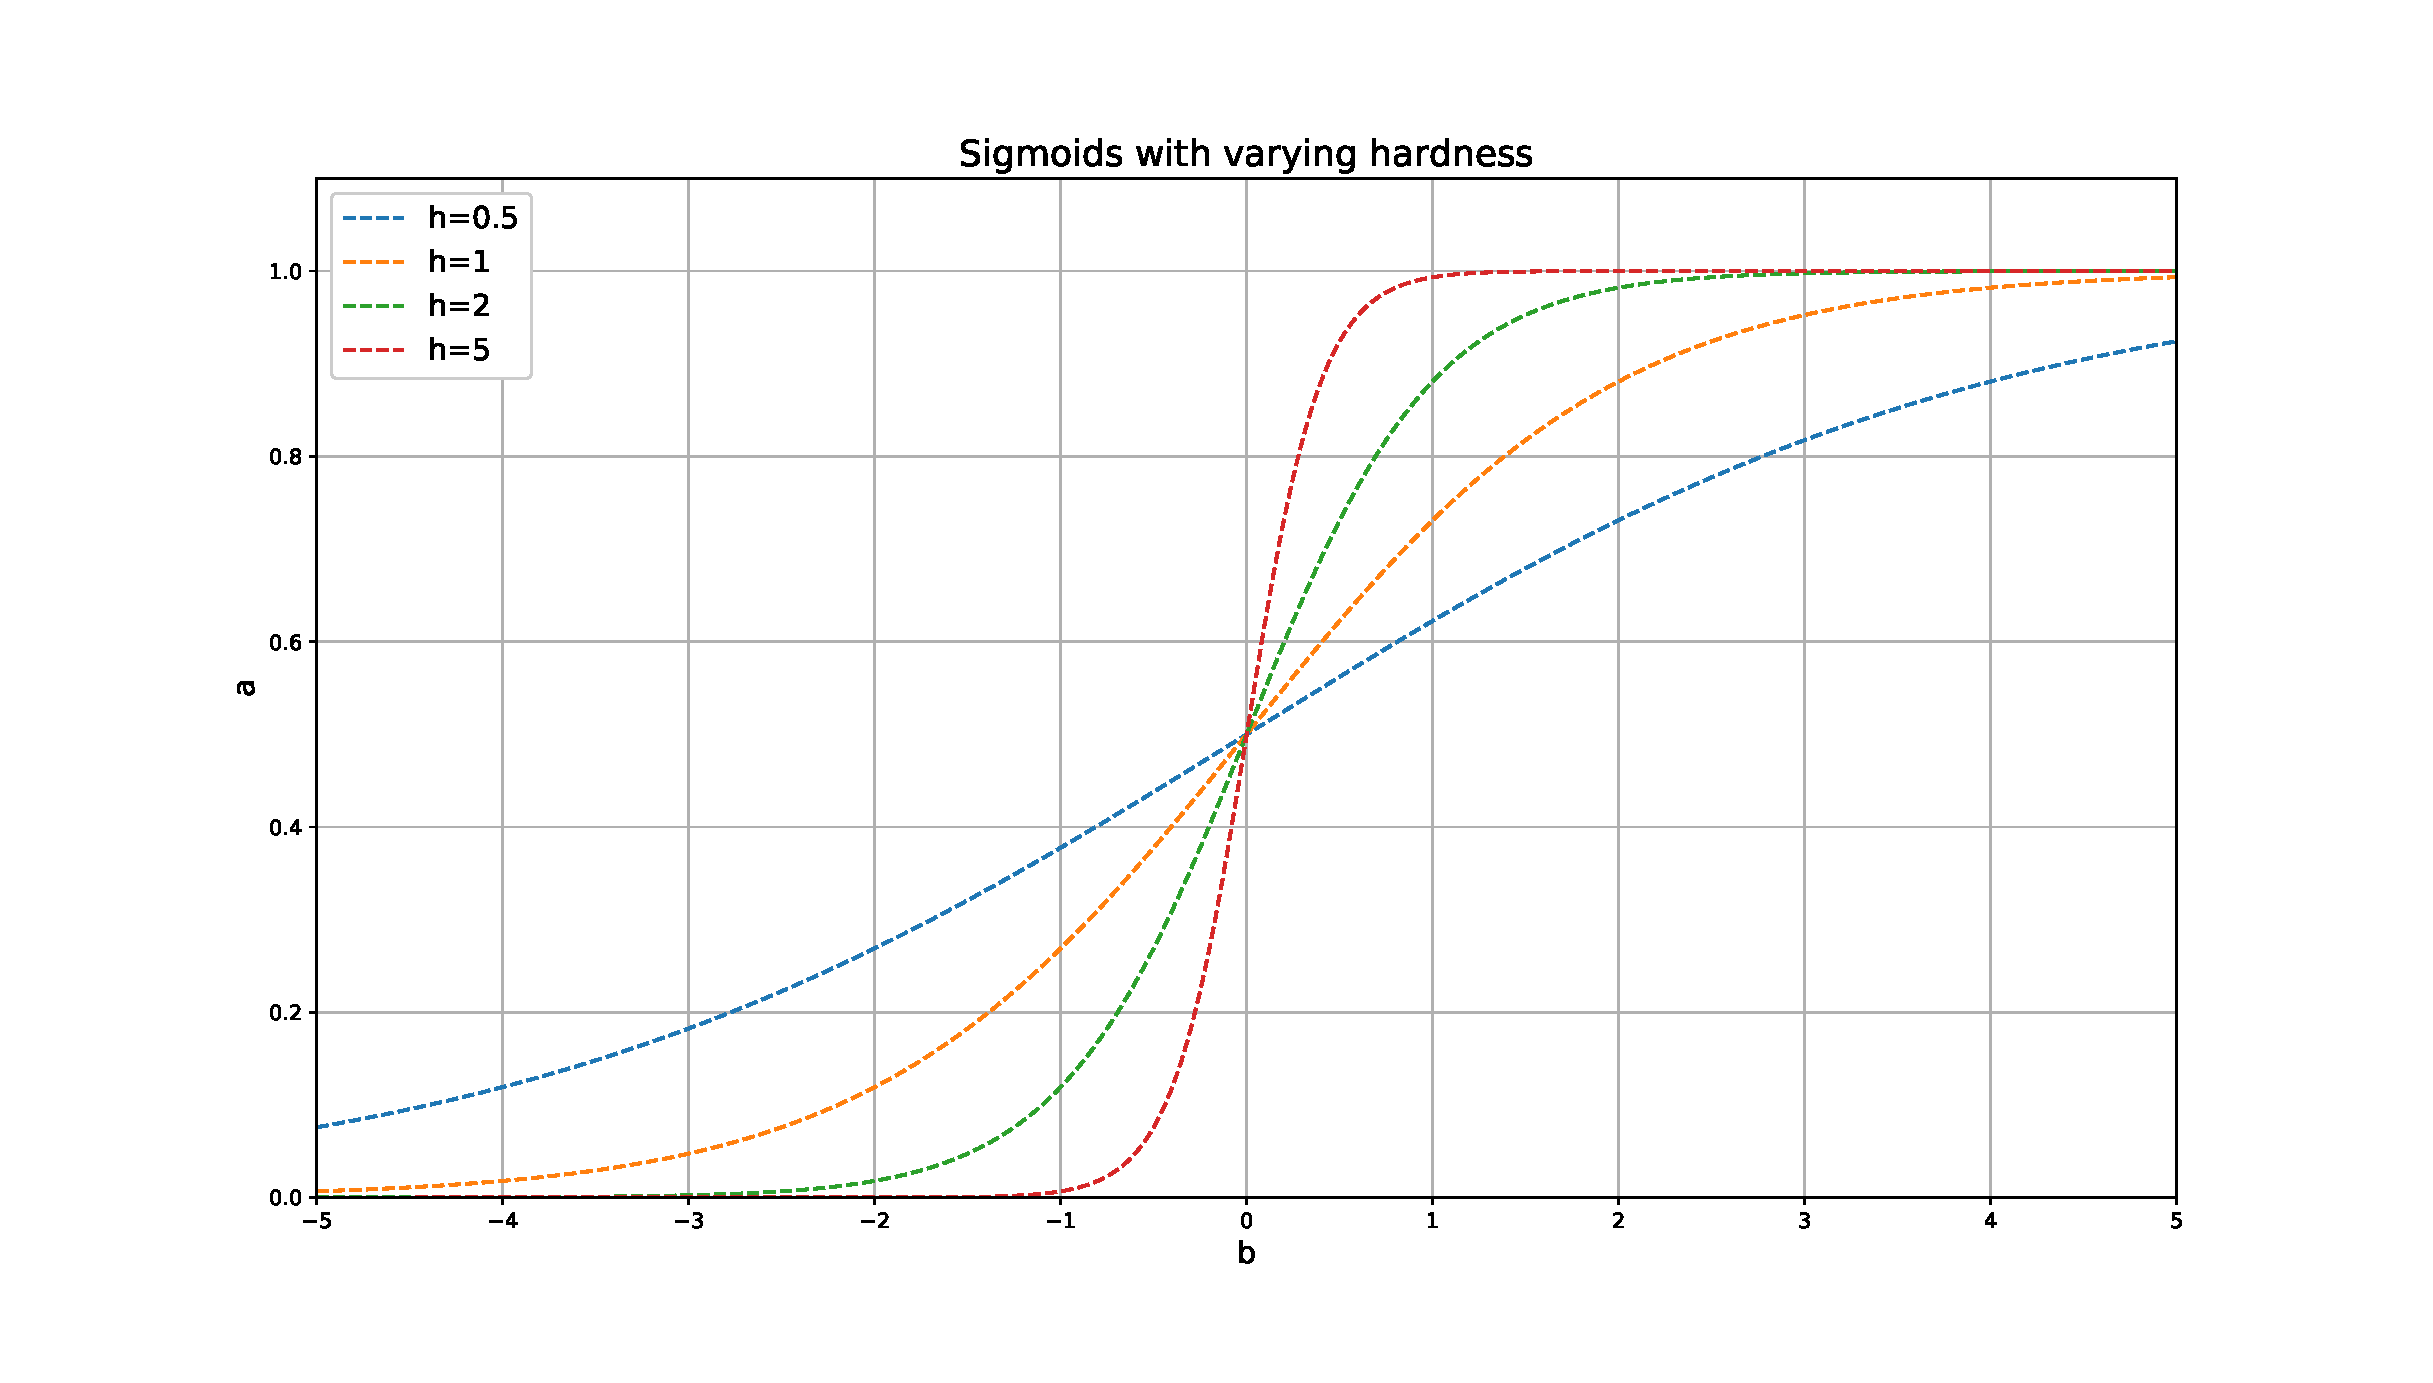
\includegraphics[width=\textwidth]{./app1/figures/sig_hard.eps}
	\caption{A 1 Dimensional Sigmoid Function with Varying Hardness Parameter}
	\label{fig:sighard}
\end{figure}

\begin{equation}
	a = \frac{1}{1 + e^{-h\cdot b}}
	\label{eqn:base_sig}
\end{equation}


Equation \ref{eqn:radsig} describes the sigmoid that we use to fit the carbon hole. In the equation, ``Counts'' is the counts in a given bin, $x$ is the horizontal raster value (in ADC bins), and $y$ is the vertical raster value (in ADC bins). For definitions of the fit parameters $p0$ through $p6$, see table \ref{tbl:sigvar_desc}. For this fit, the conversion factors are restricted to positive numbers in a small region around an ``educated guess'' of the approximate conversion factors. These ``educated guesses'' can be determined by roughly measuring, by eye, the approximate width of the carbon hole in \textit{ADC bins} and then dividing by $2mm$. The center values are restricted to the approximate range of the raster data. These restrictions ensure that the fit is not fooled by any outlying data, which can be readily determined by eye when the fit is drawn. The sign of the calibration needs to be applied (multiplicatively) to ensure the calibration is done correctly.

\begin{equation}
\mathrm{Counts} = \frac{p0}{1+e^{-p5*\left(\left(p1*\left(p2-x\right)\right)^{2}+\left(p3*\left(p4-y\right)\right)^{2}-1\right)}}+p6
\label{eqn:radsig}
\end{equation}

\begin{center}
\begin{tabulary}{0.9\textwidth}{|L|L|}
	\multicolumn{2}{c}{\textbf{Parameter Definitions}}
	\\
	\hline
	$p0$ & Approximate signal level outside the carbon hole (measured in ADC bins)\\
	$p1$ & Current (ADC bins) to $mm$ conversion factor for Horizontal Raster\\
	$p2$ & Horizontal center of the carbon hole in current (ADC) units\\
	$p3$ & Current (ADC bins) to $mm$ conversion factor for Vertical Raster\\
	$p4$ & Vertical center of the carbon hole in current (ADC) units\\
	$p5$ & ``Hardness'' factor for the sigmoid (approaches a step function as this increases)\\
	$p6$ & Approximate signal level inside the carbon hole (measured in ADC bins)\\
	\hline
\end{tabulary}
\label{tbl:sigvar_desc}
\end{center}

Note that in equation \ref{eqn:radsig}, the fit conversion factor will have units of $mm/$\textit{ADC bin}. The resulting conversion factors must be divided by 1000 before further use. This was done for clarity as the size of the Carbon Hole is typically discussed in $mm$. To avoid the need for further unit conversion, the following equation can be used instead.

\begin{equation}
\mathrm{Counts} = \frac{p0}{1+e^{-p5*\left(\left(p1*\left(p2-x\right)\right)^{2}+\left(p3*\left(p4-y\right)\right)^{2}-10^{-6}\right)}}+p6
\label{eqn:radsig_m}
\end{equation}

\begin{figure}
	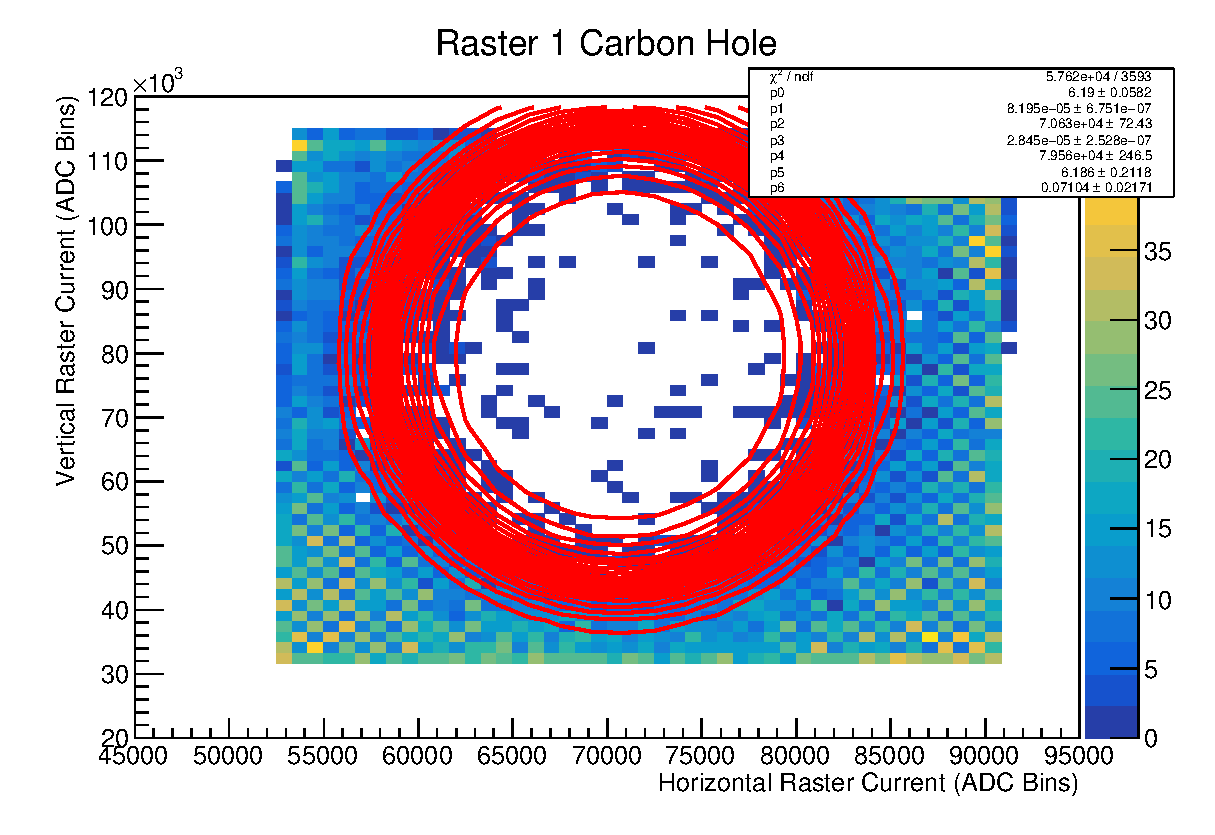
\includegraphics[width=\textwidth]{./app1/figures/hole_fit.eps}
	\caption{Using the radial sigmoid function to fit the hole in the Carbon Hole target. In this plot, the density of red rings is directly correlated to the slope of the function at that point. Where the rings are densest is the 50\% position, corresponding to where the fit locates the edge of the hole.}
	\label{fig:carbholefit}
\end{figure}

Upon further analysis, it was determined that this calibration method yielded little improvement over the ``traditional'' method. The fit places the edge of the hole at the horizontal zero-crossing of the sigmoid function. Due to smearing from the spectrometer, this is not the ``true edge'' of the hole. This was determined by looking at the physics values that the raster calibration affects. For the horizontal rasters, this is the reconstructed z position at the target. For the vertical rasters, this is W$^2$. When the rasters are properly calibrated, there should be no correlations between the raster current and the physics variables that are affected by the calibration.

Proceeding further, we determined that we ought to look at these physics values for improving the calibration. Utilizing two ``bad'' calibrations, we looked at the strength of the correlation as it is related to the calibration. If we assume that the relation is linear, we can interpolate (or extrapolate if they were bad in the same direction) to determine the correct calibration.\cite{Rey}

For the horizontal raster, we used the single carbon foil target and plot the horizontal raster current versus the reconstructed z position. We can then take slices of this plot in horizontal raster current bins and fit the resulting plots with a Gaussian and plot the peaks. With a properly calibrated raster, there should be no correlation between horizontal raster current and reconstructed z. Using two improper horizontal calibrations, we measured the slopes of the correlations. We then interpolated to determine the calibration that would yield a slope of 0. This procedure forces the sign of the calibration to be built into the answer, there is no need to apply it.

In practice, this does not yield a calibration with a slope of \textit{precisely} zero. This is due to statistical fluctuations in the data around the true correlation line. We attempted to iterate this procedure, but it did not yield significant improvement on the results.

\begin{figure}
	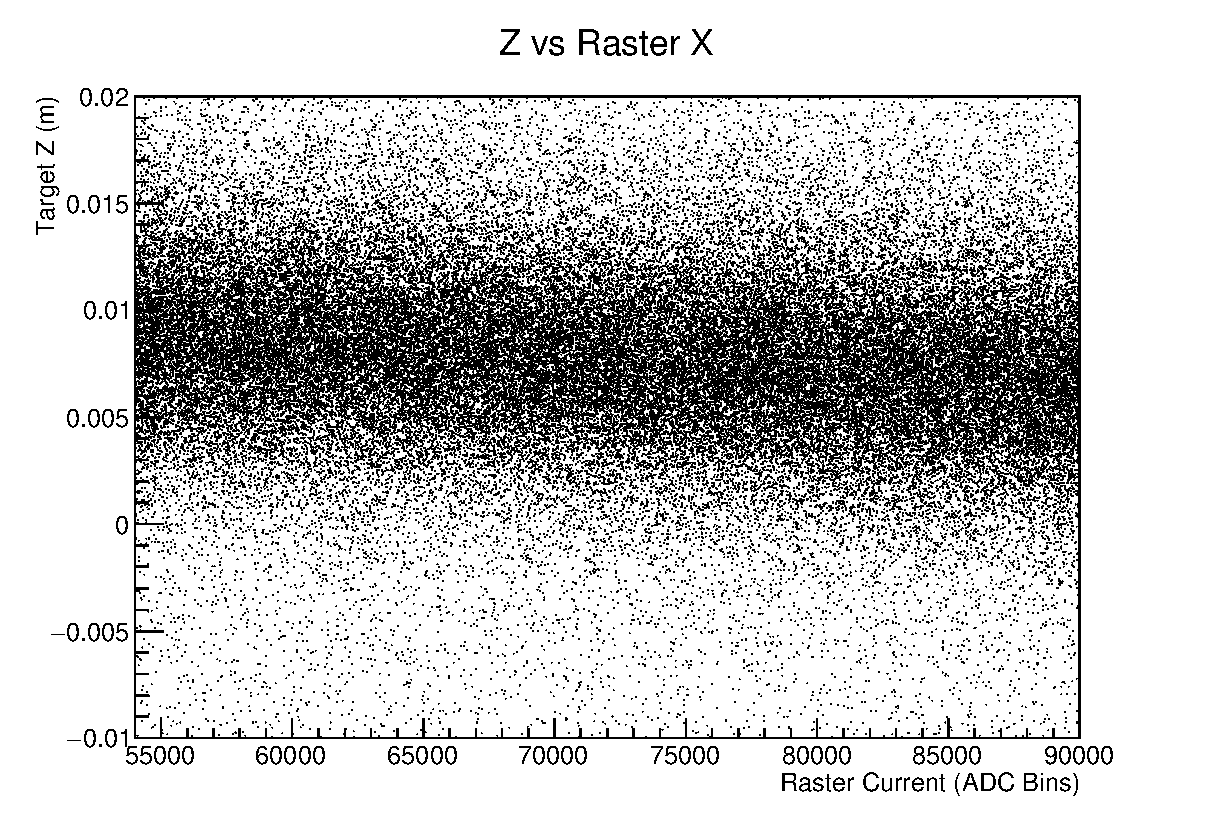
\includegraphics[width=\textwidth]{./app1/figures/old1_zvx.eps}
	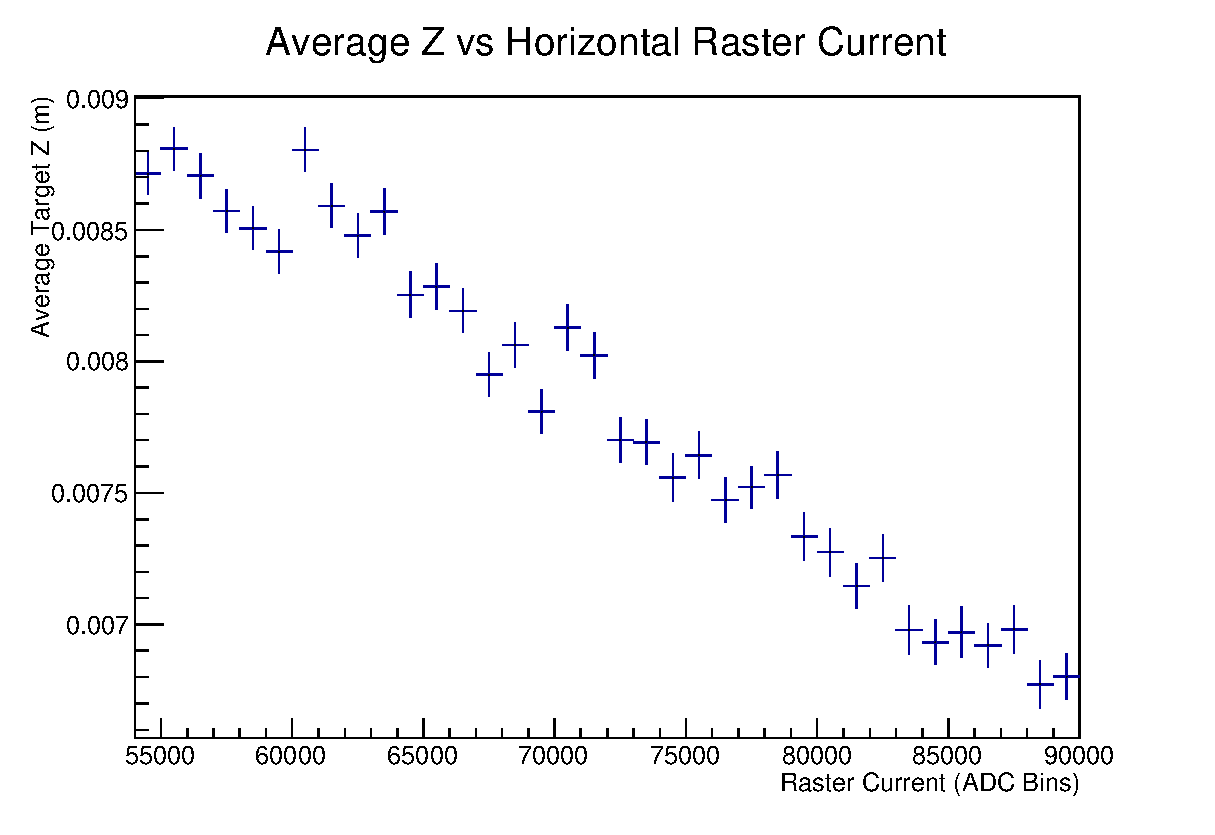
\includegraphics[width=\textwidth]{./app1/figures/old1_avgzvx_nofit.eps}
	\caption{Slices in horizontal raster current of the reconstructed z versus raster current plot are fit with a Gaussian. The peaks of the Gaussian are then plotted to see the correlation. In the plot of average z, it can be seen that the peak position shifts by over 2mm over the movement of the raster. The carbon foil is only 0.25mm thick.}
\end{figure}

\begin{figure}
	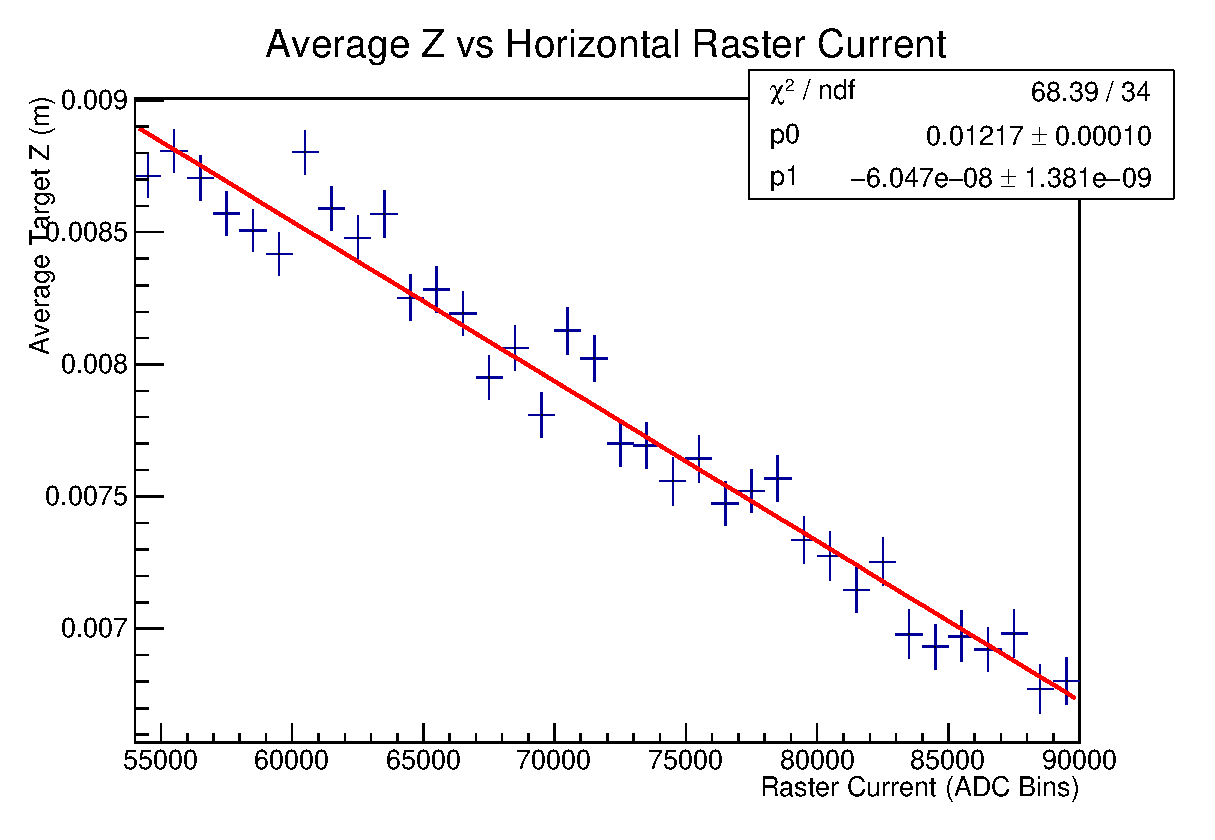
\includegraphics[width=\textwidth]{./app1/figures/old1_avgzvx.eps}
	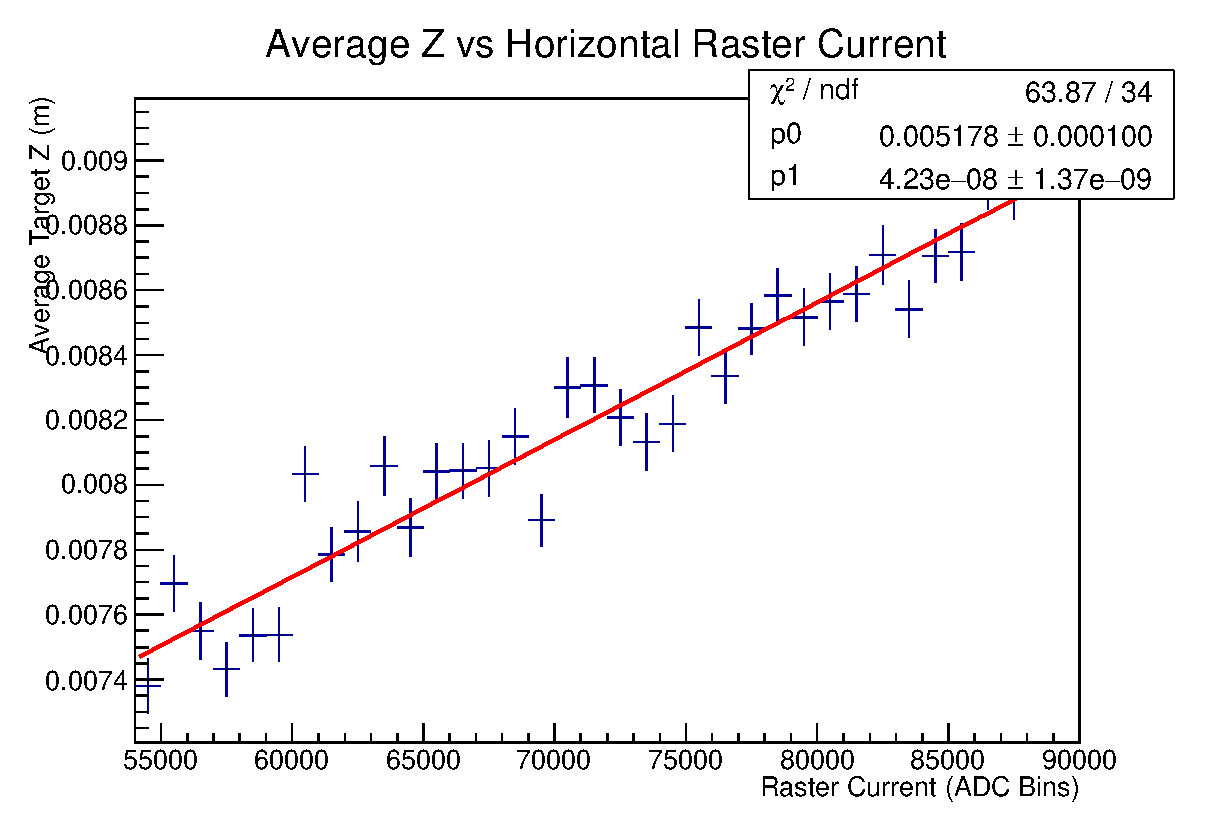
\includegraphics[width=\textwidth]{./app1/figures/old2_avgzvx.eps}
	\caption{Two ``bad'' calibrations are fit to find the correlation between horizontal raster current and the average x position. Both of these calibrations show a displacement larger than the thickness of the target.}
\end{figure}
\begin{figure}
	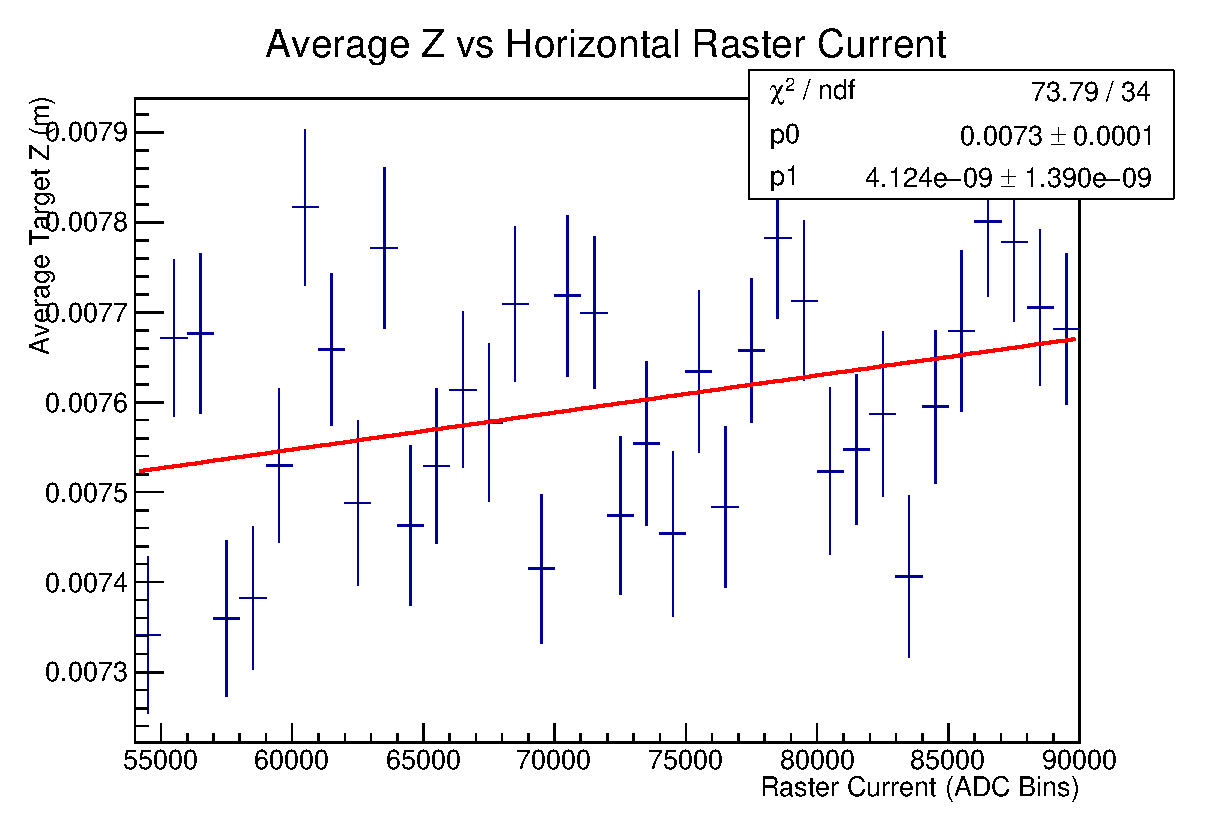
\includegraphics[width=\textwidth]{./app1/figures/avgzvx.eps}
	\caption{Using a linear fit of the correlation between average z and horizontal raster current for two ``bad'' calibrations, we can interpolate to the correct calibration. Here we can see that the shift is approximately 0.1mm.}
\end{figure}

For the vertical raster, we look for a momentum feature that the experiment can see. In the case of many of the Tritium era experiments, the Hydrogen elastic peak was measured. Plotting the vertical raster current versus the W$^2$ of Hydrogen elastic events, we followed a similar procedure to that of the horizontal raster. As with the horizontal calibration, there is no need to apply the sign of the calibration in this method.

For experiments that do not have an identifiable momentum feature, an approximation of the correct vertical calibration can be found using the horizontal calibration and the sigmoid fit of the carbon hole. Since it is known that the true calibration lies somewhere on the sigmoid above the zero-crossing, we can use the horizontal calibration to determine where that point is. To do this, we determine how many horizontal ADC bins away from center the ``true edge'' lies using the calibration determined using the z vertex reconstruction (the ``true edge'' is $1mm$ away from the center). We then evaluate equation \ref{eqn:radsig} using this value. Then, equation \ref{eqn:radsig} is reversed to determine the vertical ADC bin displacement to yield the same value. Once we have the displacement, a new vertical calibration can be determined. This is an imperfect solution, but ultimately should provide the best calibration possible in the absence of a momentum feature.

Once these methods are used to determine the slope of the raster calibration, we turn our attention back to the BPMs. The BPMs, after calibration with the harp, provide a very accurate reading of the mean beam position at their location in the beamline. This information can then be used to determine the mean position of the beam at the target. To do this, we plot each BPMs position spectrums and determine the mean value. Each spectrum must have its mean determined independently because the BPM readings lag behind events, the position is only accurate when averaged over time. Once we know the mean positions at each BPM, a track through the means can be projected to the mean position at the target.

With the slope of the raster calibrations and a point on the calibration lines (the mean position at the target), we have all the information that we need to determine the raster calibration lines. Using a simple point-slope form, we input the information for each raster and solve for the intercept.

\section{Calibrating the Beam Position at the BPMs}

The beam position must also be calibrated at the BPMs. To do this, we use the ``traditional'' method of raster calibration. As in determining the mean position at the target, the raster and BPM spectrums are plotted. The means and RMS of each spectrum are then calculated. In these cases, since we are determining the calibration at the BPMs, no projection is needed.

To determine the size calibration, the slope of the calibration line, divide the RMS of the BPM spectrum by the RMS of the raster spectrum and then multiply by the sign of the calibration. To then determine the calibration offset, point-slope form of a line can be implemented using the mean positions and the aforementioned slope calculation.\cite{Barak}